\documentclass{beamer}

\mode<presentation>
{
  \usetheme{Warsaw}
  \useoutertheme{infolines}
  \usecolortheme[RGB={28,13,151}]{structure}
  %\usetheme[height=7mm]{Rochester}
  % or ...

  \setbeamercovered{invisible}
  % or whatever (possibly just delete it)
}

\usepackage{multicol}
\usepackage{verbatim} 
\usepackage{listings}
\usepackage{tikz}
\usetikzlibrary{arrows}
\usetikzlibrary{shapes}
\tikzstyle{block}=[draw opacity=0.7,line width=1.4cm]

\lstloadlanguages{C++}
\lstnewenvironment{code}
	{%\lstset{	numbers=none, frame=lines, basicstyle=\small\ttfamily, }%
	 \csname lst@SetFirstLabel\endcsname}
	{\csname lst@SaveFirstLabel\endcsname}
\lstset{% general command to set parameter(s)
	language=C++, basicstyle=\footnotesize\ttfamily, keywordstyle=\slshape,
	emph=[1]{tipo,usa}, emphstyle={[1]\sffamily\bfseries},
	morekeywords={tint,forn,forsn},
	basewidth={0.47em,0.40em},
	columns=fixed, fontadjust, resetmargins, xrightmargin=5pt, xleftmargin=15pt,
	flexiblecolumns=false, tabsize=2, breaklines,	breakatwhitespace=false, extendedchars=true,
	numbers=left, numberstyle=\tiny, stepnumber=1, numbersep=9pt,
	frame=l, framesep=3pt,
}

\usepackage[spanish]{babel}
% or whatever

\usepackage[latin1]{inputenc}
% or whatever

\usepackage{times}
\usepackage[T1]{fontenc}
% Or whatever. Note that the encoding and the font should match. If T1
% does not look nice, try deleting the line with the fontenc.


\title{Sorting}  % (optional, use only with long paper titles)


\author[Melanie Sclar] % (optional, use only with lots of authors)
{~Melanie Sclar}
% - Give the names in the same order as the appear in the paper.
% - Use the \inst{?} command only if the authors have different
%   affiliation.
\institute[UBA] % (optional, but mostly needed)
{
  %\inst{1}
  Facultad de Ciencias Exactas y Naturales\\
  Universidad de Buenos Aires
}
\date[Octubre 2014] % (optional, should be abbreviation of conference name)
{Octubre 2014}

% Ac� se puede insertar el logo de la UBA
% \pgfdeclareimage[height=0.5cm]{university-logo}{university-logo-filename}
% \logo{\pgfuseimage{university-logo}}



% Delete this, if you do not want the table of contents to pop up at
% the beginning of each subsection:
\AtBeginSubsection[]
{
  \begin{frame}{Contenidos}
  \footnotesize
  \begin{multicols}{2} 
    \tableofcontents[currentsection, currentsubsection]
  \end{multicols}
  \end{frame}
}

\DeclareMathOperator*{\mimin}{min}
\DeclareMathOperator*{\mimax}{max}

% If you wish to uncover everything in a step-wise fashion, uncomment
% the following command: 

%\beamerdefaultoverlayspecification{<+->}


\begin{document}
\pgfdeclarelayer{background}
\pgfsetlayers{background,main}
\begin{frame}
  \titlepage
\end{frame}


\begin{frame}{El problema}

  \begin{block}{Ejercicio 18, Pr�ctica 7 de Algoritmos y Estructuras de Datos II}
Se desea ordenar los datos generados por un sensor industrial que monitorea la presencia de una sustancia en un proceso qu�mico. 

Cada una de estas mediciones es un n�mero entero. Dada la naturaleza del proceso se sabe que, dada una secuencia de n mediciones, a lo sumo $\lfloor \sqrt{n} \rfloor$ valores est�n fuera del rango $[20,40]$.
Proponer un algoritmo $O(n)$ que permita ordenar ascendentemente una secuencia de mediciones y justificar la complejidad del algoritmo propuesto.
  \end{block}
  
\end{frame}

\begin{frame}{�Nos mintieron?}

\begin{itemize}
\item En la te�rica vieron que cualquier algoritmo determin�stico basado en comparaciones (s�lo trataremos algoritmos de este tipo en la materia) realiza $\Omega( n \lg n )$ comparaciones en el peor caso.
\item Pero entonces, �C�mo puede ser posible que ordenemos un arreglo (en este caso, la lista de las mediciones del sensor) en $O(n)$?
\pause
\item Lo que ocurre es que \textbf{el teorema vale s�lo si no sabemos absolutamente nada sobre la distribuci�n de los datos de la entrada}, y este no es el caso.
\end{itemize}
    
\end{frame}

\begin{frame}{Recordando definiciones}

\begin{block}{Definici�n de parte entera}
La {\it parte entera} de un n�mero $x$ (o {\it floor function}) es el mayor entero que es menor o igual a $x$, y la representamos con $\lfloor x \rfloor$. 
\end{block}

\begin{itemize}
\item Por ejemplo, $\lfloor 5,7 \rfloor = 5$, $\lfloor 41 \rfloor = 41$, $\lfloor 0,8 \rfloor = 0$.
\item En el caso de nuestro problema, esto significa que por ejemplo, si $n = 107$, como $\sqrt{107} = 10,344...$, tenemos que $\lfloor \sqrt{107} \rfloor = 10$. Esto significa que hay a lo sumo 10 elementos fuera del intervalo $[20,40]$, pero por supuesto, no necesariamente debe haber exactamente 10 (podr�a haber menos).
\end{itemize}

\end{frame}

\begin{frame}{Un ejemplo}

\begin{itemize}
\item Yendo a nuestro problema, y para dimensionarnos la cantidad de elementos que habr� en el intervalo $[20,40]$:
\begin{itemize}
\item Como hay a lo sumo $\lfloor \sqrt{n} \rfloor$ fuera de $[20,40]$, sabemos que hay al menos $n - \lfloor \sqrt{n} \rfloor $ elementos en el intervalo nombrado.
\item Esto significa que si por ejemplo $n = 1000000$, en el rango $[20,40]$ habr� al menos $1000000 - \lfloor \sqrt{1000000} \rfloor = 999000$ elementos. Es decir, �Una enorme mayor�a!
\item {\bf La gran mayor�a de los elementos en nuestro problema se encuentra en un rango de 21 n�meros. Esto implica que si n es muy grande, los n�meros dentro de [20,40] aparecer�n repetidos muchas veces.}
\end{itemize}
\end{itemize}

\end{frame}

\begin{frame}{Counting Sort}

\begin{itemize}
\item Primero concentr�monos en resolver c�mo ordenar los elementos en el rango [20,40]. Como hay numerosos elementos, nos ser� �til el algoritmo de {\it Counting Sort}.
\end{itemize}

\begin{block}{Counting Sort}
{\it Counting sort} es un algoritmo de ordenamiento donde se cuenta la cantidad de veces que aparece cada elemento para luego ordenarlos. El ordenamiento consiste en imprimir los elementos en orden, la cantidad de veces que aparecieren en el arreglo original. 
\end{block}

\begin{itemize}
\item S�lo puede ser utilizado para ordenar elementos que sean contables (como los n�meros enteros en un determinado intervalo, pero no los n�meros reales, por ejemplo).
\end{itemize}

\end{frame}

\begin{frame}
\begin{itemize}
\item Ya resuelto el ordenamiento de los n\'umeros en [20,40], �c\'omo ordenamos lo dem\'as?
\pause
\item Lo clave es ver que faltan ordenar a lo sumo $\lfloor \sqrt{n} \rfloor$ elementos...
\item ... y conocemos algoritmos de sorting en $O(m^2)$ si $m$ es el tama\~no de la entrada.
\item Como $m \leq \lfloor \sqrt{n} \rfloor$, �podremos ordenar esto en O(n)!
\end{itemize}
\end{frame}

\begin{frame}{Pseudoc�digo}
\begin{itemize}
\item Para mayor claridad, dividimos en menores de 20, entre 20 y 40 y mayores a 40.
\end{itemize}

\begin{center}
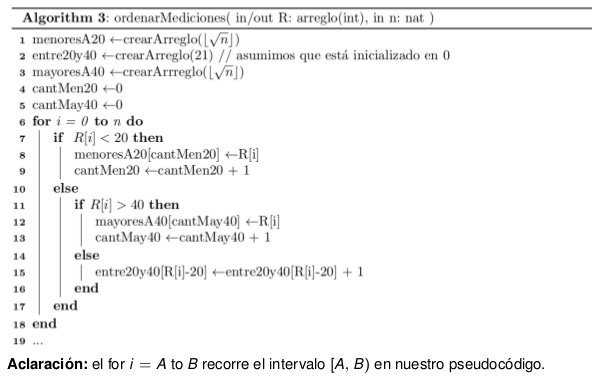
\includegraphics[scale=0.5]{codigo_top.png}
\end{center}

\end{frame}

\begin{frame}

\begin{center}
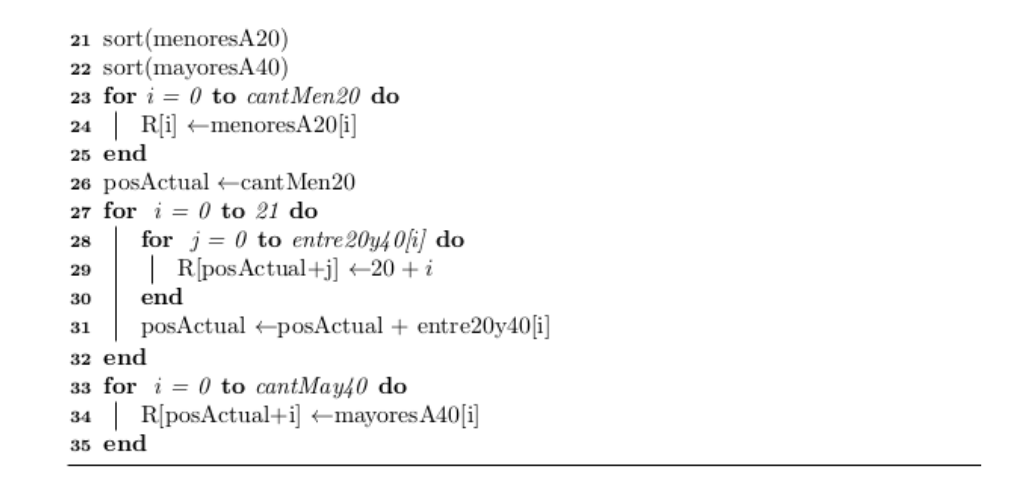
\includegraphics[scale=0.3]{codigo_bottom.png}
\end{center}

\begin{itemize}
\item Primero ordenamos los menores a 20 y los volcamos al arreglo R.
\item Luego imprimimos nuestro Counting Sort, y $posActual$ guarda la pr\'oxima posici\'on
del arreglo a escribir.
\item Finalmente ordenamos los mayores a 40 y los volcamos al arreglo R, cuidando de escribir en la posici\'on indicada
por $posActual$.
\end{itemize}
\end{frame}

\begin{frame}{Referencias}
   \begin{itemize}
   \item Introduction to Algorithms, 2nd Edition. MIT Press. Thomas H. Cormen, Charles E. Leiserson, Ronald L. Rivest, Clifford Stein.
   {\it 8.2 Counting Sort.}
  \end{itemize}
\end{frame}


\end{document}
